% !TeX root = ..\main.tex
%%%%%%%%%%%%%%%%%%%%%%%%%  

\section{Kiểm thử đơn vị (Unit testing)}
\subsection{Phương pháp thực hiện}

Bản thân ngôn ngữ Golang có hỗ trợ thư viện \textbf{testing} để viết test, do đó nhóm sử dụng thư viện này để viết các bộ testcase.\\

Nhóm thực hiện unit test cho các service trong hệ thống để đảm bảo tính đúng đắn của mã nguồn từ mức thấp nhất và kiểm tra mức độ bao phủ của unit test với mã nguồn (hay còn được gọi là coverage). Code coverage là một thông số cho biết mức độ mà mã nguồn đã được bao phủ bởi test, được ghi dưới dạng phần trăm câu lệnh đã được kiểm tra đi qua. Đây là một số thông số quan trọng để xác định mức độ tin cậy của mã, thể hiện rằng các testcase đã bao gồm đủ các trường hợp, các luồng đi trong mã hay chưa. Nhóm đặt ra yêu cầu cho code coverage của mỗi service là ít nhất 90\% để đảm bảo chất lượng mã trong mỗi service.\\



Nhóm tiến hành viết unit test cho các hàm, viết các bộ testcase cho hàm. Bộ testcase bao gồm:
\begin{itemize}
    \item Tên (name): mô tả về kết quả đầu ra mong muốn và trường hợp mà testcase sẽ đi qua.
    \item Các tham số cần thiết (args): các tham số mà hàm đang test cần.
    \item Kết quả mong đợi (want): kết quả mong muốn nhận được sau khi chạy testcase trên hàm. Trường này có thể có hoặc không.
    \item Lỗi mong đợi (wantErr): hàm trả về có lỗi hay không, true là có lỗi, false là không có lỗi. Trường này có thể có hoặc không.
\end{itemize}



Tại đây, nhóm đã đưa ra ví dụ về việc viết unit test cho một hàm. Đây là unit test cho hàm ánh xạ dữ liệu của hàng hóa thuộc đơn hàng. Hàm sẽ tiếp nhận dữ liệu đọc từ cơ sở dữ liệu và ánh xạ cũng như tính toán các trường cần thiết. Các testcase mà nhóm xây dựng cho hàm này như sau:\\


\newpage

\begin{figure}[!htp]
    \begin{center}
        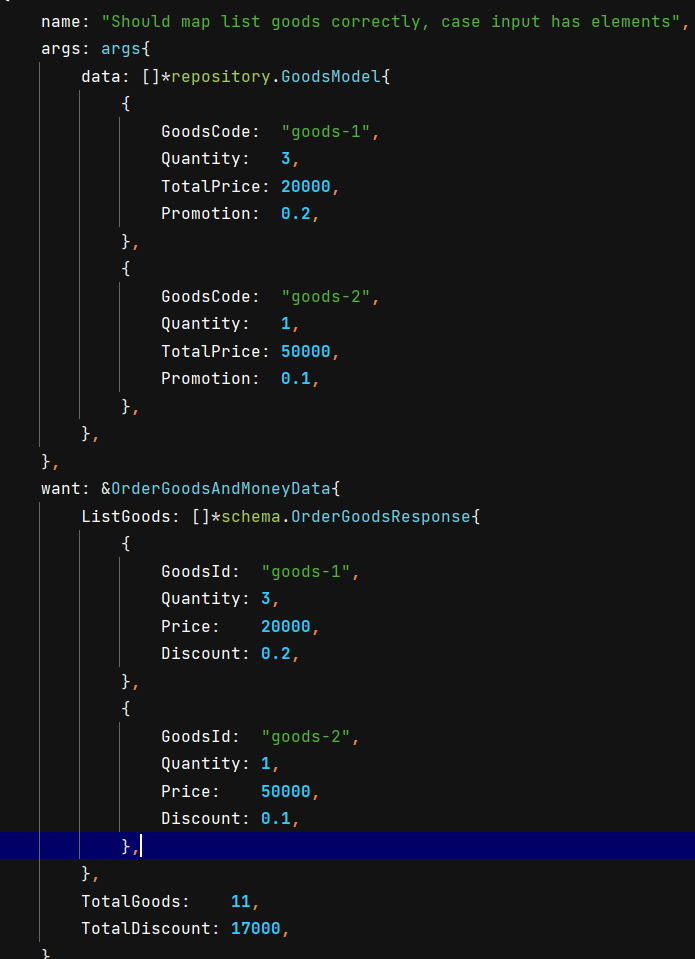
\includegraphics[width=10cm]{img/testing/unit_tc1.PNG}
    \end{center}
    \caption{Định nghĩa testcase cho unit test - Trường hợp mapping với dữ liệu đầu vào tồn tại}
\end{figure}


Testcase này kiểm tra việc ánh xạ chính xác dữ liệu đầu vào với các trường đầu ra và đảm bảo kết quả tính toán các trường \emph{TotalGoods} và \emph{TotalDiscount} theo công thức đề ra.\\


\begin{figure}[!htp]
    \begin{center}
        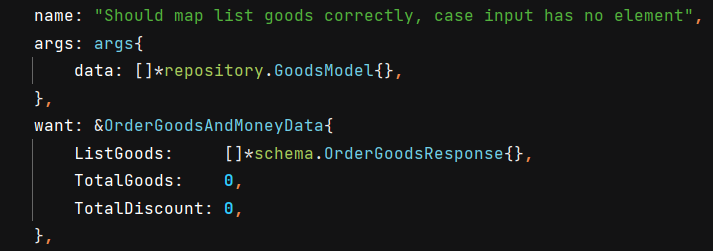
\includegraphics[width=10cm]{img/testing/unit_tc2.PNG}
    \end{center}
    \caption{Định nghĩa testcase cho unit test - Trường hợp dữ liệu đầu vào trống}
\end{figure}

Testcase này bao quát một trường hợp ngách (edge case), đó là dữ liệu đầu vào trống. Với trường hợp này, mong muốn đầu ra là danh sách hàng hóa rỗng và các trường \emph{TotalGoods}, \emph{TotalDiscount} đều là 0.\\


Để chạy test cho service, đứng tại folder của service và chạy lệnh
\begin{lstlisting}
    make test
\end{lstlisting}

Lúc đó tất cả các unit test trong service đều được chạy và kết quả sau cùng sẽ được in ra. Ví dụ với service đơn hàng, kết quả kiểm tra được in ra như sau:

\begin{lstlisting}
PASS
coverage: 90.1% of statements
ok      store-bpel/order_service/internal/controller    0.006s
\end{lstlisting}

Tương tự với các service khác, nhóm thu được kết quả test và kết quả coverage của tất cả các service.


\subsection{Kết quả kiểm thử}
{
    \setlength\extrarowheight{6pt}
    \begin{longtable}{| p{4cm}| p{4cm}| p{4cm}| p{4cm} |}
        \hline
        \textbf{Service} &  \textbf{Số testcase}  & \textbf{Coverage} & \textbf{Kết quả} \\
        \hline
        %%%%%%%%%%%%%%%%%%%%%%%%%%%%%%%%
        Account Service  &  38  & 93.3\%            & PASS             \\
        \hline
        %%%%%%%%%%%%%%%%%%%%%%%%%%%%%%%%
        Branch Service  &  20  & 93.3\%            & PASS             \\
        \hline
        %%%%%%%%%%%%%%%%%%%%%%%%%%%%%%%%
        Cart Service  &  16   & 91.2\%            & PASS             \\
        \hline
        %%%%%%%%%%%%%%%%%%%%%%%%%%%%%%%%
        Customer Service  &  14  & 93.3\%            & PASS             \\
        \hline
        %%%%%%%%%%%%%%%%%%%%%%%%%%%%%%%%
        Event Service  &   25   & 93.3\%            & PASS             \\
        \hline
        %%%%%%%%%%%%%%%%%%%%%%%%%%%%%%%%
        Goods Service  &   53   & 90.3\%            & PASS             \\
        \hline
        %%%%%%%%%%%%%%%%%%%%%%%%%%%%%%%%
        Order Service  &   35   & 90.1\%            & PASS             \\
        \hline
        %%%%%%%%%%%%%%%%%%%%%%%%%%%%%%%%
        Staff Service  &  33   & 91.3\%            & PASS             \\
        \hline
        %%%%%%%%%%%%%%%%%%%%%%%%%%%%%%%%
        Statistic Service  & 17 & 95.2\%            & PASS             \\
        \hline
        %%%%%%%%%%%%%%%%%%%%%%%%%%%%%%%%
        Warehouse Service  &  27  & 92.3\%            & PASS             \\
        \hline
        %%%%%%%%%%%%%%%%%%%%%%%%%%%%%%%%
        \caption{Kết quả của kiểm thử đơn vị}
    \end{longtable}
}

Có thể thấy tất cả service đều pass unit test và coverage đảm bảo lớn hơn 90\%, thỏa yêu cầu nhóm đề ra. Do đó, ứng dụng đó đã qua bước kiểm thử đơn vị.

\newpage
\section{Kiểm thử tích hợp (Integration testing)}
\subsection{Phương pháp thực hiện}

Sau khi thực hiện kiểm thử đơn vị cho các đơn vị nhỏ nhất của hệ thống, nhóm tiến hành kiểm thử tích hợp để đảm bảo các thành phần khi kết hợp lại sẽ hoạt động tốt và đúng như kỳ vọng. Nhóm thực hiện kiểm thử tích hợp trên các API của các service trong hệ thống. Điều này đảm bảo độ chính xác và tin cậy của các API được xuất ra từ các service. Nhóm sẽ kiểm thử các API của service với các bộ testcase bao gồm:
\begin{itemize}
    \item Tên API: tên testcase, chức năng mô tả của API mà testcase hướng tới.
    \item Đầu API: đường dẫn của API đang test.
    \item Input: dữ liệu đầu vào.
    \item Mong đợi: kết quả mong đợi của testcase.
    \item Kết quả: kết quả nhận được từ API.
\end{itemize}

Với mỗi bộ testcase, nhóm tạo tập dữ liệu mẫu trong cơ sở dữ liệu để xác định kết quả mong đợi và kiểm tra kết quả thực nhận. Để chạy các testcase, nhóm sử dụng ứng dụng Postman để gọi tới API của các service. Nhóm định nghĩa đầu API muốn kiểm tra, thêm dữ liệu đầu vào và gọi để xem kết quả mà API trả về. Với các API hoặc tác vụ có cập nhật dữ liệu vào cơ sở dữ liệu, cần kiểm tra lại dữ liệu trong cơ sở dữ liệu sau khi kiểm tra để đảm bảo dữ liệu đúng như kỳ vọng.\\

Nhóm đưa ra ví dụ để kiểm thử các API lấy thông tin người dùng bằng id và thêm người dùng. Nhóm đầu tiên tạo ra dữ liệu mẫu trong cơ sở dữ liệu của service người dùng, bảng customer:



\begin{figure}[!htp]
    \begin{center}
        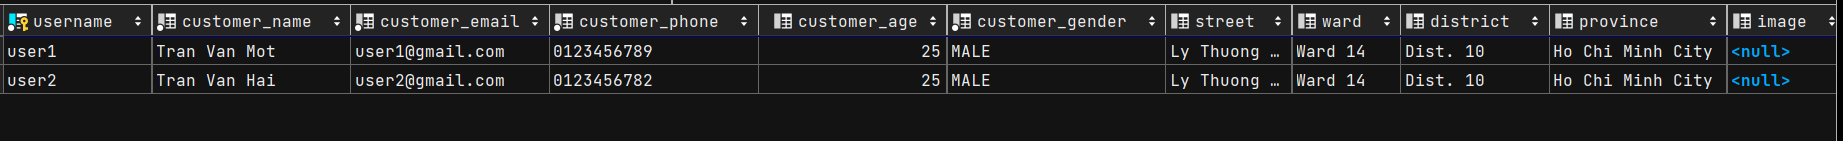
\includegraphics[width=15cm]{img/testing/sample_db.PNG}
    \end{center}
    \caption{Data mẫu được tạo ra}
\end{figure}

\newpage
\begin{itemize}
    \item API lấy thông tin người dùng.
          \begin{itemize}
              \item API: GET /api/customer-service/customer/\{username\}
              \item Input: username = user1
              \item Mong đợi:

                    \begin{figure}[!htp]
                        \begin{center}
                            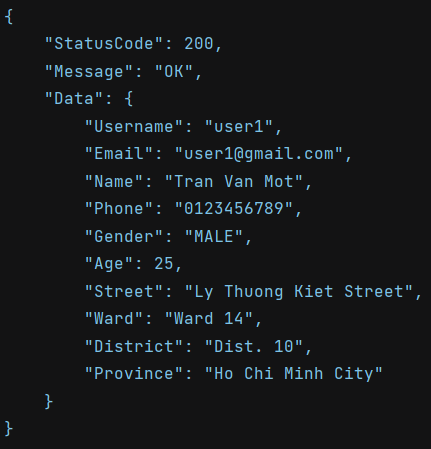
\includegraphics[width=10cm]{img/testing/inte_expected_1.PNG}
                        \end{center}
                        \caption{Kết quả mong đợi}
                    \end{figure}

                    \newpage
              \item Kêt quả: Kết quả việc gọi API bằng Postman:\\
                    \begin{figure}[!htp]
                        \begin{center}
                            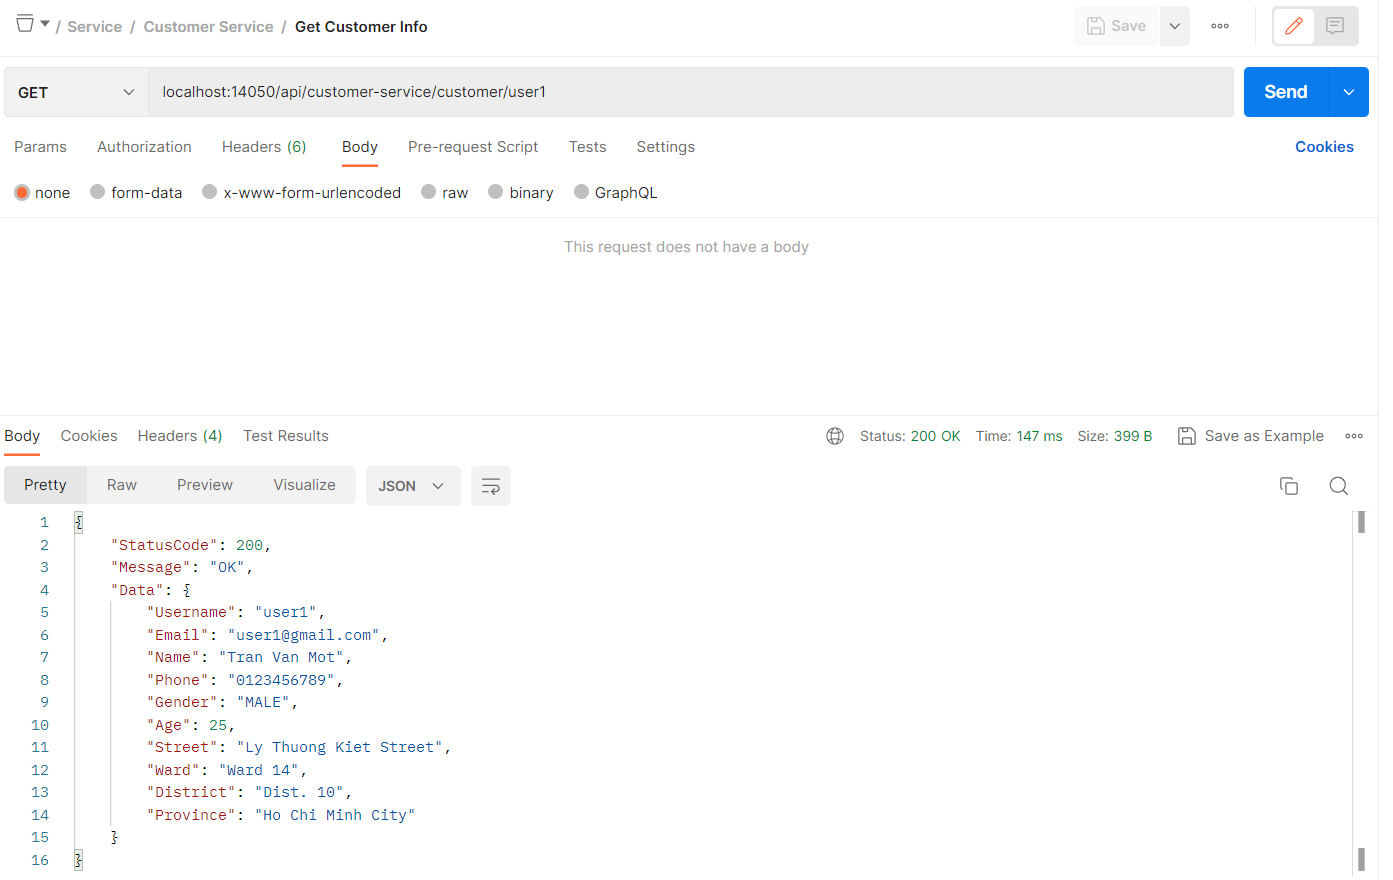
\includegraphics[width=15cm]{img/testing/inte_get_customer.PNG}
                        \end{center}
                        \caption{Gọi API lấy thông tin người dùng bằng Postman}
                    \end{figure}

                    Kết quả đầu ra đúng với kết quả mong đợi.
          \end{itemize}
    \item API thêm người dùng.
          \begin{itemize}
              \item Đầu API: POST /api/customer-service/customer
              \item Input:
                    \begin{figure}[!htp]
                        \begin{center}
                            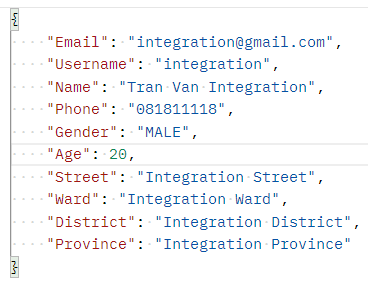
\includegraphics[width=10cm]{img/testing/inte_input_2.PNG}
                        \end{center}
                        \caption{Dữ liệu đầu vào cho testcase của API thêm người dùng }

                    \end{figure}
              \item Mong đợi: người dùng được thêm thành công vào trong cơ sở dữ liệu đúng với đầu vào.
              \item Kết quả: kết quả việc gọi API bằng Postman và dữ liệu trong cơ sở dữ liệu sau khi gọi:\\

                    \begin{figure}[!htp]
                        \begin{center}
                            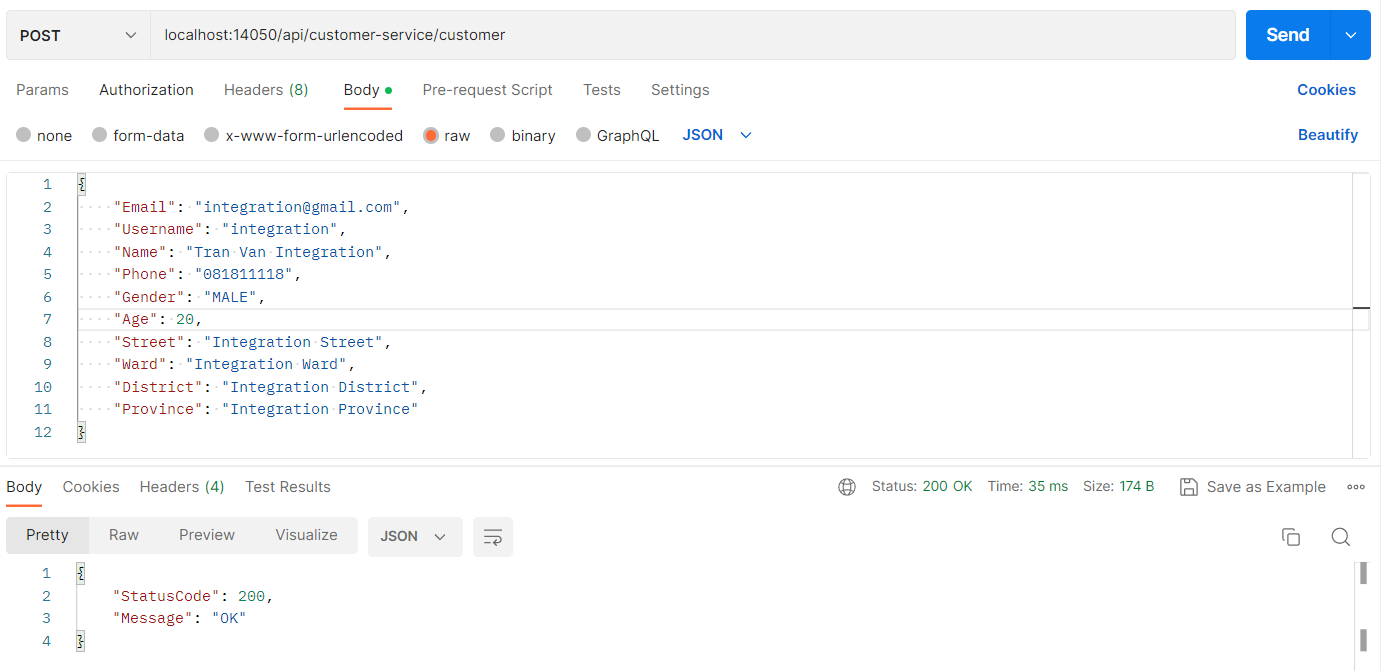
\includegraphics[width=15cm]{img/testing/inte_got_2.PNG}
                        \end{center}
                        \caption{Gọi API thêm người dùng bằng Postman}
                    \end{figure}
                    \begin{figure}[!htp]
                        \begin{center}
                            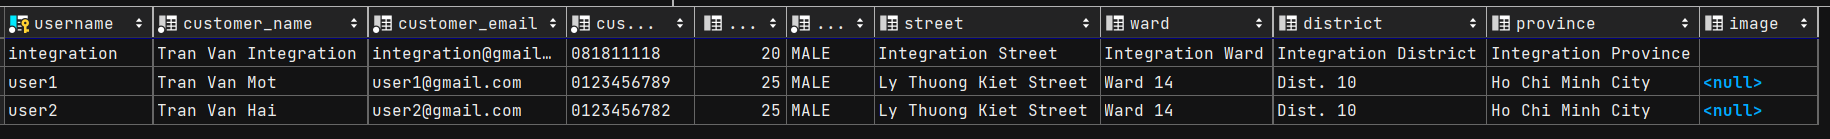
\includegraphics[width=15cm]{img/testing/inte_got_db_2.PNG}
                        \end{center}
                        \caption{Dữ liệu trong cơ sở dữ liệu sau khi gọi API}
                    \end{figure}
                    Kết quả đầu ra đúng với kết quả mong đợi.
          \end{itemize}
\end{itemize}

\subsection{Kết quả kiểm thử}
Nhóm tiến hành tạo các data mẫu và thực hiện kiểm thử các API và service còn lại tương tự như các ví dụ trên. Kết quả đầu ra đúng như kỳ vọng cho từng API và cho tất cả các service. Do đó, ứng dụng đã qua bước kiểm thử tích hợp.

\newpage
\section{Kiểm thử hệ thống (System testing)}
\subsection{Phương pháp thực hiện}

Use case testing là một phương pháp kiểm thử phần mềm tập trung vào các tình huống sử dụng cụ thể của ứng dụng. Đây là một phương pháp kiểm thử hướng đối tượng, nó tập trung vào việc kiểm tra các chức năng và tính năng của phần mềm từ góc độ của người dùng. Cụ thể, use case testing được sử dụng để kiểm tra xem liệu phần mềm có hoạt động đúng như các kịch bản sử dụng mà người dùng mong đợi hay không.\\

Các use case được xác định trong quá trình phân tích yêu cầu phần mềm, nó mô tả một chuỗi các hành động và tình huống mà người dùng sẽ thực hiện để sử dụng phần mềm. Use case testing sử dụng các kịch bản này để kiểm tra hành vi của phần mềm trong các tình huống khác nhau. Nó có thể giúp đảm bảo rằng phần mềm được xây dựng để đáp ứng các yêu cầu của người dùng và hoạt động đúng như kỳ vọng.\\

Vì vậy, nhóm chọn sử dụng phương pháp Use-case testing để kiểm thử cho hệ thống mà nhóm đã phát triển. Với use case testing, nhóm phát triển có thể đảm bảo rằng ứng dụng sẽ được hoạt động đúng như kỳ vọng và đáp ứng các yêu cầu của người dùng. Nó là một phương pháp kiểm thử quan trọng và hiệu quả để đảm bảo tính toàn vẹn, độ tin cậy và hiệu quả của phần mềm.\\

\hspace*{0.5cm}Nhóm thực hiện kiểm thử trong môi trường sau đây:
\\
{
\setlength\extrarowheight{6pt}
\begin{longtable}{| p{.30\textwidth} | p{.40\textwidth} |}
    \hline
    \textbf{Hệ điều hành}       & Window 10 64-bit          \\
    \hline
    %%%%%%%%%%%%%%%%%%%%%%%%%%%%%%%%
    \textbf{Trình duyệt}        & Google Chrome version 112 \\
    %%%%%%%%%%%%%%%%%%
    \hline
    \textbf{Phương pháp}        & Use-case testing          \\
    \hline
    \textbf{Cách thức kiểm thử} & Thủ công                  \\
    \hline
    %%%%%%%%%%%%%%%%%%%%%%%%%%%%%%%%
    \caption{Môi trường thực hiện kiểm thử hệ thống}
\end{longtable}
}

\subsection{Đặt hàng trực tuyến}

\subsubsection{Xem danh sách các sản phẩm}
{
    \setlength\extrarowheight{6pt}
    \begin{longtable}{| p{2.5cm}| p{1cm}| p{5.5cm}| p{4.5cm} | p{1.5cm} |}
        \hline
        \textbf{Test case}                                                                       & \textbf{Step name} & \textbf{Step descriptions} & \textbf{Expected Result} & \textbf{Result} \\
        \hline
        %%%%%%%%%%%%%%%%%%%%%%%%%%%%%%%%
        \multirow[t]{2}{2.5cm}{Xem danh sách tất cả sản phẩm}                                    &
        1                                                                                        &
        Truy cập vào trang chủ của hệ thống                                                      &
        Hệ thống hiển thị trang chủ của hệ thống                                                 &
        Đạt                                                                                                                                                                                     \\
        %%%%%%%%%%%%%%%%%%
        \cline{2-5}
                                                                                                 & 2                  &
        Chọn vào "Sản phẩm"                                                                      &
        Hệ thống hiển thị toàn bộ sản phẩm có bán trong cửa hàng                                 &
        Đạt                                                                                                                                                                                     \\
        \hline
        %%%%%%%%%%%%%%%%%%%%%%%%%%%%%%%%
        %%%%%%%%%%%%%%%%%%%%%%%%%%%%%%%%
        \multirow[t]{2}{2.5cm}{Xem danh sách sản phẩm nổi bật}                                   &
        1                                                                                        &
        Truy cập vào trang chủ của hệ thống                                                      &
        Hệ thống hiển thị trang chủ của hệ thống, bên trong có các sản phẩm nổi bật của hệ thống &
        Đạt                                                                                                                                                                                     \\
        %%%%%%%%%%%%%%%%%%
        \hline
        %%%%%%%%%%%%%%%%%%%%%%%%%%%%%%%%
        \caption{Kịch bản kiểm thử xem danh sách các sản phẩm}
    \end{longtable}
}

\subsubsection{Lọc sản phẩm theo đặc điểm}
{
    \setlength\extrarowheight{6pt}
    \begin{longtable}{| p{2.5cm}| p{1cm}| p{5.5cm}| p{4.5cm} | p{1.5cm} |}
        \hline
        \textbf{Test case}                                                             & \textbf{Step name} & \textbf{Step descriptions} & \textbf{Expected Result} & \textbf{Result} \\
        \hline
        %%%%%%%%%%%%%%%%%%%%%%%%%%%%%%%%
        \multirow[t]{2}{2.5cm}{Lọc sản phẩm theo đặc điểm trong trang tất cả sản phẩm} &
        1                                                                              &
        Truy cập vào trang chủ của hệ thống                                            &
        Hệ thống hiển thị trang chủ của hệ thống                                       &
        Đạt                                                                                                                                                                           \\
        %%%%%%%%%%%%%%%%%%
        \cline{2-5}
                                                                                       & 2                  &
        Chọn vào "Sản phẩm"                                                            &
        Hệ thống hiển thị toàn bộ sản phẩm có bán trong cửa hàng                       &
        Đạt                                                                                                                                                                           \\
        %%%%%%%%%%%%%%%%%%%%%%%%%%%%%%%%
        \cline{2-5}
                                                                                       & 3                  &
        Chọn vào ô "Giới tính"                                                         &
        Hệ thống hiển thị các lựa chọn về giới tính                                    &
        Đạt                                                                                                                                                                           \\
        %%%%%%%%%%%%%%%%%%%%%%%%%%%%%%%%
        \cline{2-5}
                                                                                       & 4                  &
        Chọn vào ô "Nam"                                                               &
        Hệ thống hiển thị các sản phẩm dành cho giới tính nam                          &
        Đạt                                                                                                                                                                           \\
        \hline
        \multirow[t]{2}{2.5cm}{Lọc sản phẩm theo đặc điểm nhanh qua header}            &
        1                                                                              &
        Truy cập vào trang chủ của hệ thống                                            &
        Hệ thống hiển thị trang chủ của hệ thống                                       &
        Đạt                                                                                                                                                                           \\
        %%%%%%%%%%%%%%%%%%
        \cline{2-5}
                                                                                       & 2                  &
        Chọn vào "Nam" trên phần header                                                &
        Hệ thống hiển thị các sản phẩm dành cho giới tính nam                          &
        Đạt                                                                                                                                                                           \\
        \hline
        %%%%%%%%%%%%%%%%%%%%%%%%%%%%%%%%
        \caption{Kịch bản kiểm thử lọc sản phẩm theo đặc điểm}
    \end{longtable}
}

\subsubsection{Lọc danh sách sản phẩm theo từ khóa}
{
    \setlength\extrarowheight{6pt}
    \begin{longtable}{| p{2.5cm}| p{1cm}| p{5.5cm}| p{4.5cm} | p{1.5cm} |}
        \hline
        \textbf{Test case}                                       & \textbf{Step name} & \textbf{Step descriptions} & \textbf{Expected Result} & \textbf{Result} \\
        \hline
        %%%%%%%%%%%%%%%%%%%%%%%%%%%%%%%%
        \multirow[t]{2}{2.5cm}{Xem danh sách tất cả sản phẩm}    &
        1                                                        &
        Truy cập vào trang chủ của hệ thống                      &
        Hệ thống hiển thị trang chủ của hệ thống                 &
        Đạt                                                                                                                                                     \\
        %%%%%%%%%%%%%%%%%%
        \cline{2-5}
                                                                 & 2                  &
        Nhập vào ô "Tìm kiếm" : "áo thun"                        &
        Hệ thống hiển thị các sản phẩm có chứa từ khóa "áo thun" &
        Đạt                                                                                                                                                     \\
        \hline
        %%%%%%%%%%%%%%%%%%%%%%%%%%%%%%%%
        \caption{Kịch bản kiểm thử lọc danh sách sản phẩm theo từ khóa}
    \end{longtable}
}

\subsubsection{Xem thông tin chi tiết sản phẩm}
{
    \setlength\extrarowheight{6pt}
    \begin{longtable}{| p{2.5cm}| p{1cm}| p{5.5cm}| p{4.5cm} | p{1.5cm} |}
        \hline
        \textbf{Test case}                                                                         & \textbf{Step name} & \textbf{Step descriptions} & \textbf{Expected Result} & \textbf{Result} \\
        \hline
        %%%%%%%%%%%%%%%%%%%%%%%%%%%%%%%%
        \multirow[t]{2}{2.5cm}{Xem thông tin chi tiết của sản phẩm}                                &
        1                                                                                          &
        Chọn vào "Sản phẩm"                                                                        &
        Hệ thống hiển thị toàn bộ sản phẩm có bán trong cửa hàng                                   &
        Đạt                                                                                                                                                                                       \\
        %%%%%%%%%%%%%%%%%%
        \cline{2-5}
                                                                                                   & 2                  &
        Chọn vào thẻ sản phẩm "GIÀY THỂ THAO MEN IS22-24502"                                       &
        Hệ thống hiển thị thông tin chi tiết của sản phẩm "GIÀY THỂ THAO MEN IS22-24502"           &
        Đạt                                                                                                                                                                                       \\
        \hline
        %%%%%%%%%%%%%%%%%%%%%%%%%%%%%%%%
        \multirow[t]{2}{2.5cm}{Xem thông tin chi tiết của sản phẩm qua giỏ hàng}                   &
        1                                                                                          &
        Chọn vào icon "Giỏ hàng" trên header                                                       &
        Hệ thống hiển thị toàn bộ sản phẩm có trong hàng                                           &
        Đạt                                                                                                                                                                                       \\
        %%%%%%%%%%%%%%%%%%
        \cline{2-5}
                                                                                                   & 2                  &
        Chọn vào thẻ tên sản phẩm "GIÀY THỂ THAO MEN IS22-24502"                                   &
        Hệ thống hiển thị thông tin chi tiết của sản phẩm "GIÀY THỂ THAO MEN IS22-24502"           &
        Đạt                                                                                                                                                                                       \\
        \hline
        %%%%%%%%%%%%%%%%%%%%%%%%%%%%%%%%
        \multirow[t]{2}{2.5cm}{Xem thông tin chi tiết của sản phẩm qua lịch sử mua hàng}           &
        1                                                                                          &
        Chọn vào icon "Đơn hàng" trên header                                                       &
        Hệ thống hiển thị toàn bộ đơn hàng chưa nhận                                               &
        Đạt                                                                                                                                                                                       \\
        %%%%%%%%%%%%%%%%%%
        \cline{2-5}
                                                                                                   & 2                  &
        Chọn vào thẻ chứa sản phẩm "GIÀY THỂ THAO MEN IS22-24502"                                  &
        Hệ thống hiển thị thông tin chi tiết đơn hàng chứa sản phẩm "GIÀY THỂ THAO MEN IS22-24502" &
        Đạt                                                                                                                                                                                       \\
        %%%%%%%%%%%%%%%%%%
        \cline{2-5}
                                                                                                   & 3                  &
        Chọn vào thẻ tên sản phẩm "GIÀY THỂ THAO MEN IS22-24502"                                   &
        Hệ thống hiển thị thông tin chi tiết của sản phẩm "GIÀY THỂ THAO MEN IS22-24502"           &
        Đạt                                                                                                                                                                                       \\
        \hline
        %%%%%%%%%%%%%%%%%%%%%%%%%%%%%%%%
        \caption{Kịch bản kiểm thử xem thông tin chi tiết sản phẩm}
    \end{longtable}
}

\subsubsection{Thêm sản phẩm vào giỏ hàng}
{
    \setlength\extrarowheight{6pt}
    \begin{longtable}{| p{2.5cm}| p{1cm}| p{5.5cm}| p{4.5cm} | p{1.5cm} |}
        \hline
        \textbf{Test case}                                                                           & \textbf{Step name} & \textbf{Step descriptions} & \textbf{Expected Result} & \textbf{Result} \\
        \hline
        %%%%%%%%%%%%%%%%%%%%%%%%%%%%%%%%
        \multirow[t]{2}{2.5cm}{Thêm sản phẩm vào giỏ hàng}                                           &
        1                                                                                            &
        Chọn vào "Sản phẩm"                                                                          &
        Hệ thống hiển thị toàn bộ sản phẩm có bán trong cửa hàng                                     &
        Đạt                                                                                                                                                                                         \\
        %%%%%%%%%%%%%%%%%%
        \cline{2-5}
                                                                                                     & 2                  &
        Chọn vào thẻ sản phẩm "GIÀY THỂ THAO MEN IS22-24502"                                         &
        Hệ thống hiển thị thông tin chi tiết của sản phẩm "GIÀY THỂ THAO MEN IS22-24502"             &
        Đạt                                                                                                                                                                                         \\
        %%%%%%%%%%%%%%%%%%
        \cline{2-5}
                                                                                                     & 3                  &
        Chọn vào thẻ màu sắc "Xanh"                                                                  &
        Hệ thống hiển thị giá cho sản phẩm "GIÀY THỂ THAO MEN IS22-24502" với màu sắc "Xanh"         &
        Đạt                                                                                                                                                                                         \\
        %%%%%%%%%%%%%%%%%%
        \cline{2-5}
                                                                                                     & 4                  &
        Chọn vào nút "+" để tăng số lượng                                                            &
        Hệ thống hiển thị tăng số lượng lên thành "2"                                                &
        Đạt                                                                                                                                                                                         \\
        %%%%%%%%%%%%%%%%%%
        \cline{2-5}
                                                                                                     & 5                  &
        Chọn vào nút "Thêm vào giỏ hàng" để thêm vào giỏ hàng                                        &
        Hệ thống hiển thị thông báo thêm vào giỏ hàng thành công                                     &
        Đạt                                                                                                                                                                                         \\
        \hline
        %%%%%%%%%%%%%%%%%%%%%%%%%%%%%%%%
        \multirow[t]{2}{2.5cm}{Thêm nhanh sản phẩm vào giỏ hàng}                                     &
        1                                                                                            &
        Chọn vào "Sản phẩm"                                                                          &
        Hệ thống hiển thị toàn bộ sản phẩm có bán trong cửa hàng                                     &
        Đạt                                                                                                                                                                                         \\
        %%%%%%%%%%%%%%%%%%
        \cline{2-5}
                                                                                                     & 2                  &
        Chọn vào nút chứa icon "Thêm vào giỏ hàng" trong thẻ sản phẩm "GIÀY THỂ THAO MEN IS22-24502" &
        Hệ thống hiển thị thông báo thêm vào giỏ hàng thành công                                     &
        Đạt                                                                                                                                                                                         \\
        \hline
        %%%%%%%%%%%%%%%%%%%%%%%%%%%%%%%%
        \multirow[t]{2}{2.5cm}{Thêm sản phẩm vào giỏ hàng từ lịch sử mua hàng}                       &
        1                                                                                            &
        Chọn vào icon "Đơn hàng" trên header                                                         &
        Hệ thống hiển thị toàn bộ đơn hàng chưa nhận                                                 &
        Đạt                                                                                                                                                                                         \\
        %%%%%%%%%%%%%%%%%%
        \cline{2-5}
                                                                                                     & 2                  &
        Chọn vào nút "Mua lại" của thẻ chứa sản phẩm "GIÀY THỂ THAO MEN IS22-24502"                  &
        Hệ thống hiển thị trang giỏ hàng và trong đó chứa thẻ "GIÀY THỂ THAO MEN IS22-24502"         &
        Đạt                                                                                                                                                                                         \\
        \hline
        %%%%%%%%%%%%%%%%%%%%%%%%%%%%%%%%
        \caption{Kịch bản kiểm thử thêm sản phẩm vào giỏ hàng}
    \end{longtable}
}

\subsubsection{Mua hàng trực tuyến}
{
    \setlength\extrarowheight{6pt}
    \begin{longtable}{| p{2.5cm}| p{1cm}| p{5.5cm}| p{4.5cm} | p{1.5cm} |}
        \hline
        \textbf{Test case}                                                                              & \textbf{Step name} & \textbf{Step descriptions} & \textbf{Expected Result} & \textbf{Result} \\
        \hline
        %%%%%%%%%%%%%%%%%%%%%%%%%%%%%%%%
        \multirow[t]{2}{2.5cm}{Mua hàng trực tuyển}                                                     &
        1                                                                                               &
        Chọn vào "Giỏ hàng" trên header                                                                 &
        Hệ thống hiển thị danh sách các sản phẩm trong giỏ hàng                                         &
        Đạt                                                                                                                                                                                            \\
        %%%%%%%%%%%%%%%%%%
        \cline{2-5}
                                                                                                        & 2                  &
        Chọn vào thẻ sản phẩm "GIÀY THỂ THAO MEN IS22-24502"                                            &
        Hệ thống hiển thị sản phẩm "GIÀY THỂ THAO MEN IS22-24502" đã được chọn                          &
        Đạt                                                                                                                                                                                            \\
        %%%%%%%%%%%%%%%%%%
        \cline{2-5}
                                                                                                        & 3                  &
        Chọn vào nút "Thanh toán"                                                                       &
        Hệ thống chuyển đến trang thanh toán cùng với thông tin sản phẩm "GIÀY THỂ THAO MEN IS22-24502" &
        Đạt                                                                                                                                                                                            \\
        %%%%%%%%%%%%%%%%%%
        \cline{2-5}
                                                                                                        & 4                  &
        Nhập dữ liệu vào biểu mẫu thanh toán:
        \begin{itemize}
            \item Tên: Trần Tuấn
            \item Số điện thoại: 0987123456
            \item Email: trantuan@gmail.com
            \item Tỉnh / thành phố: Bình Dương
            \item Quận / huyện: Dĩ An
            \item Phường / xã: Đông Hòa
            \item Số nhà, đường: 151 Lương Định của
            \item Chọn "Thanh toán trực tiếp"
            \item Chọn chấp nhận chính sách
        \end{itemize}
                                                                                                        &
        Hệ thống hiển thị giá vận chuyển và tổng đơn hàng                                               &
        Đạt                                                                                                                                                                                            \\
        %%%%%%%%%%%%%%%%%%
        \cline{2-5}
                                                                                                        & 5                  &
        Chọn vào nút "Đặt hàng" để đặt hàng                                                             &
        Hệ thống hiển thị thông báo đặt hàng thành công                                                 &
        Đạt                                                                                                                                                                                            \\
        \hline
        %%%%%%%%%%%%%%%%%%%%%%%%%%%%%%%%
        \multirow[t]{2}{2.5cm}{Đặt hàng nhưng chưa có sản phẩm trong giỏ hàng}                          &
        1                                                                                               &
        Chọn vào "Giỏ hàng" trên header                                                                 &
        Hệ thống hiển thị "Bạn chưa có sản phẩm nào trong giỏ hàng."                                    &
        Đạt                                                                                                                                                                                            \\
        %%%%%%%%%%%%%%%%%%
        \cline{2-5}
                                                                                                        & 2                  &
        Chọn vào nút "Xem sản phẩm"                                                                     &
        Hệ thống hiển thị trang sản phẩm cho người dùng                                                 &
        Đạt                                                                                                                                                                                            \\
        %%%%%%%%%%%%%%%%%%
        \cline{2-5}
                                                                                                        & 3                  &
        Chọn vào nút icon "Thêm vào giỏ hàng" thẻ sản phẩm "GIÀY THỂ THAO MEN IS22-24502"               &
        Hệ thống thông báo thêm vào giỏ hàng thành công                                                 &
        Đạt                                                                                                                                                                                            \\
        %%%%%%%%%%%%%%%%%%
        \cline{2-5}
                                                                                                        & 4                  &
        Chọn vào "Giỏ hàng" trên header                                                                 &
        Hệ thống hiển thị danh sách các sản phẩm trong giỏ hàng                                         &
        Đạt                                                                                                                                                                                            \\
        %%%%%%%%%%%%%%%%%%
        \cline{2-5}
                                                                                                        & 5                  &
        Chọn vào thẻ sản phẩm "GIÀY THỂ THAO MEN IS22-24502"                                            &
        Hệ thống hiển thị sản phẩm "GIÀY THỂ THAO MEN IS22-24502" đã được chọn                          &
        Đạt                                                                                                                                                                                            \\
        %%%%%%%%%%%%%%%%%%
        \cline{2-5}
                                                                                                        & 6                  &
        Chọn vào nút "Thanh toán"                                                                       &
        Hệ thống chuyển đến trang thanh toán cùng với thông tin sản phẩm "GIÀY THỂ THAO MEN IS22-24502" &
        Đạt                                                                                                                                                                                            \\
        %%%%%%%%%%%%%%%%%%
        \cline{2-5}
                                                                                                        & 7                  &
        Nhập dữ liệu vào biểu mẫu thanh toán:
        \begin{itemize}
            \item Tên: Trần Tuấn
            \item Số điện thoại: 0987123456
            \item Email: trantuan@gmail.com
            \item Tỉnh / thành phố: Bình Dương
            \item Quận / huyện: Dĩ An
            \item Phường / xã: Đông Hòa
            \item Số nhà, đường: 151 Lương Định của
            \item Chọn "Thanh toán trực tiếp"
            \item Chọn chấp nhận chính sách
        \end{itemize}
                                                                                                        &
        Hệ thống hiển thị giá vận chuyển và tổng đơn hàng                                               &
        Đạt                                                                                                                                                                                            \\
        %%%%%%%%%%%%%%%%%%
        \cline{2-5}
                                                                                                        & 8                  &
        Chọn vào nút "Đặt hàng" để đặt hàng                                                             &
        Hệ thống hiển thị thông báo đặt hàng thành công                                                 &
        Đạt                                                                                                                                                                                            \\
        \hline
        %%%%%%%%%%%%%%%%%%%%%%%%%%%%%%%%
        \multirow[t]{2}{2.5cm}{Người dùng không muốn hoàn tất đặt hàng}                                 &
        1                                                                                               &
        Chọn vào "Giỏ hàng" trên header                                                                 &
        Hệ thống hiển thị danh sách các sản phẩm trong giỏ hàng                                         &
        Đạt                                                                                                                                                                                            \\
        %%%%%%%%%%%%%%%%%%
        \cline{2-5}
                                                                                                        & 2                  &
        Chọn vào thẻ sản phẩm "GIÀY THỂ THAO MEN IS22-24502"                                            &
        Hệ thống hiển thị sản phẩm "GIÀY THỂ THAO MEN IS22-24502" đã được chọn                          &
        Đạt                                                                                                                                                                                            \\
        %%%%%%%%%%%%%%%%%%
        \cline{2-5}
                                                                                                        & 3                  &
        Chọn vào nút "Thanh toán"                                                                       &
        Hệ thống chuyển đến trang thanh toán cùng với thông tin sản phẩm "GIÀY THỂ THAO MEN IS22-24502" &
        Đạt                                                                                                                                                                                            \\
        %%%%%%%%%%%%%%%%%%
        \cline{2-5}
                                                                                                        & 4                  &
        Nhập dữ liệu vào biểu mẫu thanh toán:
        \begin{itemize}
            \item Tên: Trần Tuấn
            \item Số điện thoại: 0987123456
            \item Email: trantuan@gmail.com
            \item Tỉnh / thành phố: Bình Dương
            \item Quận / huyện: Dĩ An
            \item Phường / xã: Đông Hòa
            \item Số nhà, đường: 151 Lương Định của
            \item Chọn "Thanh toán trực tiếp"
            \item Chọn chấp nhận chính sách
        \end{itemize}
                                                                                                        &
        Hệ thống hiển thị giá vận chuyển và tổng đơn hàng                                               &
        Đạt                                                                                                                                                                                            \\
        %%%%%%%%%%%%%%%%%%
        \cline{2-5}
                                                                                                        & 5                  &
        Chọn vào logo trang web trên header để không hoàn tất đặt hàng                                  &
        Hệ thống hiển thị trang chủ                                                                     &
        Đạt                                                                                                                                                                                            \\
        \hline
        %%%%%%%%%%%%%%%%%%%%%%%%%%%%%%%%
        \caption{Kịch bản kiểm thử mua hàng trực tuyến}
    \end{longtable}
}

\subsection{Quản lý sự kiện}

\subsubsection{Xem thông tin chi tiết sự kiện}
{
    \setlength\extrarowheight{6pt}
    \begin{longtable}{| p{2.5cm}| p{1cm}| p{5.5cm}| p{4.5cm} | p{1.5cm} |}
        \hline
        \textbf{Test case}                           & \textbf{Step name} & \textbf{Step descriptions}           & \textbf{Expected Result}                         & \textbf{Result} \\
        \hline
        %%%%%%%%%%%%%%%%%%%%%%%%%%%%%%%%
        \multirow[c]{2}{2.5cm}{Xem chi tiết sự kiện} & 1                  & Truy cập hệ thống quản lý sự kiện    & Hệ thống hiển thị danh sách sự kiện              & Đạt             \\
        %%%%%%%%%%%%%%%%%%
        \cline{2-5}
                                                     & 2                  & Chọn vào sự kiện "Sale hè năng động" & Hệ thống hiển thị thông tin chi tiết của sự kiện & Đạt             \\
        \hline
        %%%%%%%%%%%%%%%%%%%%%%%%%%%%%%%%
        \caption{Kịch bản kiểm thử xem thông tin chi tiết sự kiện}
    \end{longtable}
}

\newpage

\subsubsection{Thêm sự kiện mới}
{
    \setlength\extrarowheight{6pt}
    \begin{longtable}{| p{2.5cm}| p{1cm}| p{5.5cm}| p{4.5cm} | p{1.5cm} |}
        \hline
        \textbf{Test case}                           & \textbf{Step name}                           & \textbf{Step descriptions}                                & \textbf{Expected Result}                                             & \textbf{Result} \\
        \hline
        %%%%%%%%%%%%%%%%%%%%%%%%%%%%%%%%
        \multirow[t]{2}{2.5cm}{Thêm sự kiện mới}     & 1                                            & Truy cập hệ thống quản lý sự kiện                         & Hệ thống hiển thị danh sách sự kiện                                  & Đạt             \\
        %%%%%%%%%%%%%%%%%%
        \cline{2-5}
                                                     & 2                                            & Chọn vào nút "Thêm mới"                                   & Hệ thống hiển thị trang thêm mới sự kiện                             & Đạt             \\
        %%%%%%%%%%%%%%%%%%
        \cline{2-5}
                                                     & 3                                            & Nhập dữ liệu vào biểu mẫu:
        \begin{itemize}
            \item Tên sự kiện: Sự kiện mới
            \item Ngày: 01/05/2023 \& 30/05/2023
            \item Mức giảm: 10
            \item Thời điểm: 00:00 \& 23:00
        \end{itemize}         & Hệ thống vẫn hiển thị trang thêm mới sự kiện & Đạt                                                                                                                                                                       \\
        \cline{2-5}
        %%%%%%%%%%%%%%%%%%
                                                     & 4                                            & Chọn vào nút "Chọn sản phẩm"                              & Hệ thống hiển thị danh sách các sản phẩm                             & Đạt             \\
        \cline{2-5}
        %%%%%%%%%%%%%%%%%%
                                                     & 5                                            & Chọn sản phẩm "Giày sneaker nam/nử 35135GW" và chọn "Lưu" & Hệ thống hiển thị trang thêm mới sự kiện với danh sách hàng vừa chọn & Đạt             \\
        \cline{2-5}
        %%%%%%%%%%%%%%%%%%
                                                     & 6                                            & Chọn vào nút "Lưu"                                        & Hệ thống hiển thị thông báo thành công                               & Đạt             \\
        \hline
        %%%%%%%%%%%%%%%%%%%%%%%%%%%%%%%%    
        \multirow[t]{2}{2.5cm}{Hủy thêm sự kiện mới} & 1                                            & Truy cập hệ thống quản lý sự kiện                         & Hệ thống hiển thị danh sách sự kiện                                  & Đạt             \\
        %%%%%%%%%%%%%%%%%%
        \cline{2-5}
                                                     & 2                                            & Chọn vào nút "Thêm mới"                                   & Hệ thống hiển thị trang thêm mới sự kiện                             & Đạt             \\
        %%%%%%%%%%%%%%%%%%
        \cline{2-5}
                                                     & 3                                            & Nhập dữ liệu vào biểu mẫu:
        \begin{itemize}
            \item Tên sự kiện: Sự kiện mới
            \item Ngày: 01/05/2023 \& 30/05/2023
            \item Mức giảm: 10
            \item Thời điểm: 00:00 \& 23:00
        \end{itemize}         & Hệ thống vẫn hiển thị trang thêm mới sự kiện & Đạt                                                                                                                                                                       \\
        \cline{2-5}
        %%%%%%%%%%%%%%%%%%
                                                     & 4                                            & Chọn vào nút "Hủy"                                        & Hệ thống hiển thị danh sách sự kiện                                  & Đạt             \\
        \hline
        %%%%%%%%%%%%%%%%%%%%%%%%%%%%%%%%
        \caption{Kịch bản kiểm thử thêm sự kiện mới}
    \end{longtable}
}


\subsubsection{Chỉnh sửa sự kiện}
{
    \setlength\extrarowheight{6pt}
    \begin{longtable}{| p{2.5cm}| p{1cm}| p{5.5cm}| p{4.5cm} | p{1.5cm} |}
        \hline
        \textbf{Test case}                            & \textbf{Step name}                           & \textbf{Step descriptions}                                     & \textbf{Expected Result}                                                     & \textbf{Result} \\
        \hline
        %%%%%%%%%%%%%%%%%%%%%%%%%%%%%%%%
        \multirow[t]{2}{2.5cm}{Chỉnh sửa sự kiện}     & 1                                            & Truy cập hệ thống quản lý sự kiện                              & Hệ thống hiển thị danh sách sự kiện                                          & Đạt             \\
        %%%%%%%%%%%%%%%%%%
        \cline{2-5}
                                                      & 2                                            & Chọn vào sự kiện "Sale phụ kiện nữ"                            & Hệ thống hiển thị trang chỉnh sửa thông tin sự kiệu                          & Đạt             \\
        %%%%%%%%%%%%%%%%%%
        \cline{2-5}
                                                      & 3                                            & Sửa dữ liệu trong biểu mẫu:
        \begin{itemize}
            \item Tên sự kiện: Sale phụ kiện nữ 123
            \item Ngày: 01/05/2023 \& 30/05/2023
            \item Mức giảm: 10
            \item Thời điểm: 00:00 \& 23:59
        \end{itemize}       & Hệ thống vẫn hiển thị trang thêm mới sự kiện & Đạt                                                                                                                                                                                       \\
        \cline{2-5}
        %%%%%%%%%%%%%%%%%%
                                                      & 4                                            & Chọn vào nút có icon thùng rác ở sản phẩm "Túi nữ NF2\_W53009" & Hệ thống vẫn hiển thị trang thêm mới sự kiện với danh sách sản phẩm thay đổi & Đạt             \\
        \cline{2-5}
        %%%%%%%%%%%%%%%%%%
                                                      & 5                                            & Chọn vào nút "Lưu"                                             & Hệ thống hiển thị thông báo thành công                                       & Đạt             \\
        \hline
        %%%%%%%%%%%%%%%%%%%%%%%%%%%%%%%%    
        \multirow[t]{2}{2.5cm}{Hủy chỉnh sửa sự kiện} & 1                                            & Truy cập hệ thống quản lý sự kiện                              & Hệ thống hiển thị danh sách sự kiện                                          & Đạt             \\
        %%%%%%%%%%%%%%%%%%
        \cline{2-5}
                                                      & 2                                            & Chọn vào sự kiện "Sale phụ kiện nữ"                            & Hệ thống hiển thị trang chỉnh sửa thông tin sự kiệu                          & Đạt             \\
        %%%%%%%%%%%%%%%%%%
        \cline{2-5}
                                                      & 3                                            & Sửa dữ liệu trong biểu mẫu:
        \begin{itemize}
            \item Tên sự kiện: Sale phụ kiện nữ 123
            \item Ngày: 01/05/2023 \& 30/05/2023
            \item Mức giảm: 10
            \item Thời điểm: 00:00 \& 23:59
        \end{itemize}       & Hệ thống vẫn hiển thị trang thêm mới sự kiện & Đạt                                                                                                                                                                                       \\
        \cline{2-5}
        %%%%%%%%%%%%%%%%%%
                                                      & 4                                            & Chọn vào nút "Hủy"                                             & Hệ thống hiển thị danh sách sự kiện                                          & Đạt             \\
        \hline
        %%%%%%%%%%%%%%%%%%%%%%%%%%%%%%%%
        \caption{Kịch bản kiểm thử chỉnh sửa sự kiện}
    \end{longtable}
}


\subsection{Quản lý chi nhánh}
\subsubsection{ Xem thông tin chi tiết chi nhánh}
{
    \setlength\extrarowheight{6pt}
    \begin{longtable}{| p{2.5cm}| p{1cm}| p{5.5cm}| p{4.5cm} | p{1.5cm} |}
        \hline
        \textbf{Test case}                                        & \textbf{Step name} & \textbf{Step descriptions}                & \textbf{Expected Result}                           & \textbf{Result} \\
        \hline
        %%%%%%%%%%%%%%%%%%%%%%%%%%%%%%%%
        \multirow[t]{2}{2.5cm}{ Xem thông tin chi tiết chi nhánh} & 1                  & Truy cập hệ thống quản lý chi nhánh       & Hệ thống hiển thị danh sách chi nhánh              & Đạt             \\
        %%%%%%%%%%%%%%%%%%
        \cline{2-5}
                                                                  & 2                  & Chọn vào chi nhánh "Chi nhánh Bình Dương" & Hệ thống hiển thị thông tin chi tiết của chi nhánh & Đạt             \\
        \hline
        %%%%%%%%%%%%%%%%%%%%%%%%%%%%%%%%
        \caption{Kịch bản kiểm thử xem thông tin chi tiết chi nhánh}
    \end{longtable}
}

\subsubsection{Thêm chi nhánh}
{
    \setlength\extrarowheight{6pt}
    \begin{longtable}{| p{2.5cm}| p{1cm}| p{5.5cm}| p{4.5cm} | p{1.5cm} |}
        \hline
        \textbf{Test case}                         & \textbf{Step name}                             & \textbf{Step descriptions}          & \textbf{Expected Result}                      & \textbf{Result} \\
        \hline
        %%%%%%%%%%%%%%%%%%%%%%%%%%%%%%%%
        \multirow[t]{2}{2.5cm}{Thêm chi nhánh}     & 1                                              & Truy cập hệ thống quản lý chi nhánh & Hệ thống hiển thị danh sách chi nhánh         & Đạt             \\
        %%%%%%%%%%%%%%%%%%
        \cline{2-5}
                                                   & 2                                              & Chọn vào nút "Thêm mới"             & Hệ thống hiển thị biểu mẫu thêm mới chi nhánh & Đạt             \\
        %%%%%%%%%%%%%%%%%%
        \cline{2-5}
                                                   & 3                                              & Nhập dữ liệu vào biểu mẫu:
        \begin{itemize}
            \item Tên chi nhánh: Chi nhánh mới
            \item Đường: Lê Văn Việt
            \item Phường: Kp.1
            \item Quận: Thủ Đức
            \item Tỉnh: Tp.Hồ Chí Minh
            \item Giờ mở cửa: 06:00
            \item Giờ đóng cửa: 23:00
        \end{itemize}         & Hệ thống vẫn hiển thị biểu mẫu thêm mới        & Đạt                                                                                                                        \\
        \cline{2-5}
        %%%%%%%%%%%%%%%%%%
                                                   & 4                                              & Chọn vào nút "Lưu"                  & Hệ thống hiển thị thông báo thành công        & Đạt             \\
        \hline
        %%%%%%%%%%%%%%%%%%%%%%%%%%%%%%%%    
        \multirow[t]{2}{2.5cm}{Hủy thêm chi nhánh} & 1                                              & Truy cập hệ thống quản lý chi nhánh & Hệ thống hiển thị danh sách chi nhánh         & Đạt             \\
        %%%%%%%%%%%%%%%%%%
        \cline{2-5}
                                                   & 2                                              & Chọn vào nút "Thêm mới"             & Hệ thống hiển thị trang thêm mới chi nhánh    & Đạt             \\
        %%%%%%%%%%%%%%%%%%
        \cline{2-5}
                                                   & 3                                              & Nhập dữ liệu vào biểu mẫu:
        \begin{itemize}
            \item Tên chi nhánh: Chi nhánh mới
            \item Đường: Lê Văn Việt
            \item Phường: Kp.1
            \item Quận: Thủ Đức
            \item Tỉnh: Tp.Hồ Chí Minh
            \item Giờ mở cửa: 06:00
            \item Giờ đóng cửa: 23:00
        \end{itemize}         & Hệ thống vẫn hiển thị trang thêm mới chi nhánh & Đạt                                                                                                                        \\
        \cline{2-5}
        %%%%%%%%%%%%%%%%%%
                                                   & 4                                              & Chọn vào nút "Hủy"                  & Hệ thống tắt biểu mẫu thêm mới                & Đạt             \\
        \hline
        %%%%%%%%%%%%%%%%%%%%%%%%%%%%%%%%
        \caption{Kịch bản kiểm thử thêm chi nhánh}
    \end{longtable}
}


\subsubsection{Chỉnh sửa chi nhánh}
{
    \setlength\extrarowheight{6pt}
    \begin{longtable}{| p{2.5cm}| p{1cm}| p{5.5cm}| p{4.5cm} | p{1.5cm} |}
        \hline
        \textbf{Test case}                              & \textbf{Step name}                           & \textbf{Step descriptions}                          & \textbf{Expected Result}                                 & \textbf{Result} \\
        \hline
        %%%%%%%%%%%%%%%%%%%%%%%%%%%%%%%%
        \multirow[t]{2}{2.5cm}{Chỉnh sửa chi nhánh}     & 1                                            & Truy cập hệ thống quản lý chi nhánh                 & Hệ thống hiển thị danh sách chi nhánh                    & Đạt             \\
        %%%%%%%%%%%%%%%%%%
        \cline{2-5}
                                                        & 2                                            & Chọn vào chỉnh sửa chi nhánh "Chi nhánh Bình Dương" & Hệ thống hiển thị biểu mẫu chỉnh sửa thông tin chi nhánh & Đạt             \\
        %%%%%%%%%%%%%%%%%%
        \cline{2-5}
                                                        & 3                                            & Sửa dữ liệu trong biểu mẫu:
        \begin{itemize}
            \item Tên chi nhánh: Chi nhánh Bình Dương 123
            \item Đường: Lê Văn Việt 123
            \item Phường: Kp.1 23
            \item Quận: Thủ Đức 123
            \item Tỉnh: Tp.Hồ Chí Minh 123
            \item Giờ mở cửa: 06:00
            \item Giờ đóng cửa: 23:00
        \end{itemize}   & Hệ thống vẫn hiển thị biểu mẫu chỉnh sửa     & Đạt                                                                                                                                                              \\
        \cline{2-5}
        %%%%%%%%%%%%%%%%%%
                                                        & 4                                            & Chọn nút "Lưu"                                      & Hệ thống hiển thị thông báo thành công                   & Đạt             \\
        \hline
        %%%%%%%%%%%%%%%%%%%%%%%%%%%%%%%%    
        \multirow[t]{2}{2.5cm}{Hủy chỉnh sửa chi nhánh} & 1                                            & Truy cập hệ thống quản lý chi nhánh                 & Hệ thống hiển thị danh sách chi nhánh                    & Đạt             \\
        %%%%%%%%%%%%%%%%%%
        \cline{2-5}
                                                        & 2                                            & Chọn vào chỉnh sửa chi nhánh "Chi nhánh Bình Dương" & Hệ thống hiển thị biểu mẫu chỉnh sửa thông tin sự kiệu   & Đạt             \\
        %%%%%%%%%%%%%%%%%%
        \cline{2-5}
                                                        & 3                                            & Sửa dữ liệu trong biểu mẫu:
        \begin{itemize}
            \item Tên chi nhánh: Chi nhánh Bình Dương 123
            \item Đường: Lê Văn Việt 123
            \item Phường: Kp.1 23
            \item Quận: Thủ Đức 123
            \item Tỉnh: Tp.Hồ Chí Minh 123
            \item Giờ mở cửa: 06:00
            \item Giờ đóng cửa: 23:00
        \end{itemize}   & Hệ thống vẫn hiển thị trang thêm mới sự kiện & Đạt                                                                                                                                                              \\
        \cline{2-5}
        %%%%%%%%%%%%%%%%%%
                                                        & 4                                            & Chọn nút "Hủy"                                      & Hệ thống tắt biểu mẫu chỉnh sửa                          & Đạt             \\
        \hline
        %%%%%%%%%%%%%%%%%%%%%%%%%%%%%%%%
        \caption{Kịch bản kiểm thử chỉnh sửa chi nhánh}
    \end{longtable}
}

\subsubsection{Xóa chi nhánh}
{
    \setlength\extrarowheight{6pt}
    \begin{longtable}{| p{2.5cm}| p{1cm}| p{5.5cm}| p{4.5cm} | p{1.5cm} |}
        \hline
        \textbf{Test case}                    & \textbf{Step name} & \textbf{Step descriptions}                & \textbf{Expected Result}                           & \textbf{Result} \\
        \hline
        %%%%%%%%%%%%%%%%%%%%%%%%%%%%%%%%
        \multirow[t]{2}{2.5cm}{Xóa chi nhánh} & 1                  & Truy cập hệ thống quản lý chi nhánh       & Hệ thống hiển thị danh sách chi nhánh              & Đạt             \\
        %%%%%%%%%%%%%%%%%%
        \cline{2-5}
                                              & 2                  & Chọn vào chi nhánh "Chi nhánh Bình Dương" & Hệ thống hiển thị thông tin chi tiết của chi nhánh & Đạt             \\
        %%%%%%%%%%%%%%%%%%
        \cline{2-5}
                                              & 3                  & Chọn nút "Xóa"                            & Hệ thống yêu cầu xác nhận                          & Đạt             \\
        \cline{2-5}
        %%%%%%%%%%%%%%%%%%
                                              & 4                  & Chọn nút "Xác nhận"                       & Hệ thống hiển thị thông báo thành công             & Đạt             \\
        \hline
        %%%%%%%%%%%%%%%%%%%%%%%%%%%%%%%%    
        \multirow[t]{2}{2.5cm}{Xóa chi nhánh} & 1                  & Truy cập hệ thống quản lý chi nhánh       & Hệ thống hiển thị danh sách chi nhánh              & Đạt             \\
        %%%%%%%%%%%%%%%%%%
        \cline{2-5}
                                              & 2                  & Chọn vào chi nhánh "Chi nhánh Bình Dương" & Hệ thống hiển thị thông tin chi tiết của chi nhánh & Đạt             \\
        %%%%%%%%%%%%%%%%%%
        \cline{2-5}
                                              & 3                  & Chọn nút "Xóa"                            & Hệ thống yêu cầu xác nhận                          & Đạt             \\
        \cline{2-5}
        %%%%%%%%%%%%%%%%%%
                                              & 4                  & Chọn nút "Hủy"                            & Hệ thống tắt yêu cầu xác nhận                      & Đạt             \\
        \hline
        %%%%%%%%%%%%%%%%%%%%%%%%%%%%%%%%
        \caption{Kịch bản kiểm thử xóa chi nhánh}
    \end{longtable}
}


\subsection{Quản lý nhân viên}
\subsubsection{ Xem thông tin chi tiết nhân viên}
{
    \setlength\extrarowheight{6pt}
    \begin{longtable}{| p{2.5cm}| p{1cm}| p{5.5cm}| p{4.5cm} | p{1.5cm} |}
        \hline
        \textbf{Test case}                                        & \textbf{Step name} & \textbf{Step descriptions}          & \textbf{Expected Result}                           & \textbf{Result} \\
        \hline
        %%%%%%%%%%%%%%%%%%%%%%%%%%%%%%%%
        \multirow[t]{2}{2.5cm}{ Xem thông tin chi tiết nhân viên} & 1                  & Truy cập hệ thống quản lý nhân viên & Hệ thống hiển thị danh sách nhân viên              & Đạt             \\
        %%%%%%%%%%%%%%%%%%
        \cline{2-5}
                                                                  & 2                  & Chọn vào nhân viên "Philip Bùi"     & Hệ thống hiển thị thông tin chi tiết của nhân viên & Đạt             \\
        \hline
        %%%%%%%%%%%%%%%%%%%%%%%%%%%%%%%%
        \caption{Kịch bản kiểm thử xem thông tin chi tiết nhân viên}
    \end{longtable}
}

\subsubsection{Thêm nhân viên}
{
    \setlength\extrarowheight{6pt}
    \begin{longtable}{| p{2.5cm}| p{1cm}| p{5.5cm}| p{4.5cm} | p{1.5cm} |}
        \hline
        \textbf{Test case}                         & \textbf{Step name}                             & \textbf{Step descriptions}          & \textbf{Expected Result}                      & \textbf{Result} \\
        \hline
        %%%%%%%%%%%%%%%%%%%%%%%%%%%%%%%%
        \multirow[t]{2}{2.5cm}{Thêm nhân viên}     & 1                                              & Truy cập hệ thống quản lý nhân viên & Hệ thống hiển thị danh sách nhân viên         & Đạt             \\
        %%%%%%%%%%%%%%%%%%
        \cline{2-5}
                                                   & 2                                              & Chọn vào nút "Thêm mới"             & Hệ thống hiển thị biểu mẫu thêm mới nhân viên & Đạt             \\
        %%%%%%%%%%%%%%%%%%
        \cline{2-5}
                                                   & 3                                              & Nhập dữ liệu vào biểu mẫu:
        \begin{itemize}
            \item Họ tên: Nhân viên mới
            \item Email: nvmoi@gmail.com
            \item Ngày sinh: 01/01/2000
            \item Điện thoại: 037462843
            \item Quê quán: Bình Dương
            \item Nơi làm việc: Chi nhánh Bình Dương
            \item Căn cước: 332857485623
            \item Vị trí: Nhân viên
            \item Giới tính: Nam
            \item Lương: 5000000
            \item Đường: Lê Văn Việt
            \item Phường: Kp.1
            \item Quận: Thủ Đức
            \item Tỉnh: Tp.Hồ Chí Minh
        \end{itemize}   & Hệ thống vẫn hiển thị biểu mẫu thêm mới        & Đạt                                                                                                                              \\
        \cline{2-5}
        %%%%%%%%%%%%%%%%%%
                                                   & 4                                              & Chọn vào nút "Lưu"                  & Hệ thống hiển thị thông báo thành công        & Đạt             \\
        \hline
        %%%%%%%%%%%%%%%%%%%%%%%%%%%%%%%%    
        \multirow[t]{2}{2.5cm}{Hủy thêm nhân viên} & 1                                              & Truy cập hệ thống quản lý nhân viên & Hệ thống hiển thị danh sách nhân viên         & Đạt             \\
        %%%%%%%%%%%%%%%%%%
        \cline{2-5}
                                                   & 2                                              & Chọn vào nút "Thêm mới"             & Hệ thống hiển thị trang thêm mới nhân viên    & Đạt             \\
        %%%%%%%%%%%%%%%%%%
        \cline{2-5}
                                                   & 3                                              & Nhập dữ liệu vào biểu mẫu:
        \begin{itemize}
            \item Họ tên: Nhân viên mới
            \item Email: nvmoi@gmail.com
            \item Ngày sinh: 01/01/2000
            \item Điện thoại: 037462843
            \item Quê quán: Bình Dương
            \item Nơi làm việc: Chi nhánh Bình Dương
            \item Căn cước: 332857485623
            \item Vị trí: Nhân viên
            \item Giới tính: Nam
            \item Lương: 5000000
            \item Đường: Lê Văn Việt
            \item Phường: Kp.1
            \item Quận: Thủ Đức
            \item Tỉnh: Tp.Hồ Chí Minh
        \end{itemize}   & Hệ thống vẫn hiển thị trang thêm mới nhân viên & Đạt                                                                                                                              \\
        \cline{2-5}
        %%%%%%%%%%%%%%%%%%
                                                   & 4                                              & Chọn vào nút "Hủy"                  & Hệ thống tắt biểu mẫu thêm mới                & Đạt             \\
        \hline
        %%%%%%%%%%%%%%%%%%%%%%%%%%%%%%%%
        \caption{Kịch bản kiểm thử thêm nhân viên}
    \end{longtable}
}


\subsubsection{Chỉnh sửa nhân viên}
{
    \setlength\extrarowheight{6pt}
    \begin{longtable}{| p{2.5cm}| p{1cm}| p{5.5cm}| p{4.5cm} | p{1.5cm} |}
        \hline
        \textbf{Test case}                          & \textbf{Step name}             & \textbf{Step descriptions}                & \textbf{Expected Result}                               & \textbf{Result} \\
        \hline
        %%%%%%%%%%%%%%%%%%%%%%%%%%%%%%%%
        \multirow[t]{2}{2.5cm}{Chỉnh sửa nhân viên} & 1                              & Truy cập hệ thống quản lý nhân viên       & Hệ thống hiển thị danh sách nhân viên                  & Đạt             \\
        %%%%%%%%%%%%%%%%%%
        \cline{2-5}
                                                    & 2                              & Chọn vào chỉnh sửa nhân viên "Philip Bùi" & Hệ thống hiển thị biểu mẫu chỉnh sửa thông tin sự kiệu & Đạt             \\
        %%%%%%%%%%%%%%%%%%
        \cline{2-5}
                                                    & 3                              & Sửa dữ liệu trong biểu mẫu:
        \begin{itemize}
            \item Họ tên: Philip Bùi 123
            \item Ngày sinh: 01/01/2000
            \item Điện thoại: 037462843
            \item Quê quán: Bình Dương
            \item Nơi làm việc: Chi nhánh Bình Dương
            \item Căn cước: 332857485623
            \item Vị trí: Nhân viên
            \item Giới tính: Nam
            \item Lương: 5000000
            \item Đường: Lê Văn Việt
            \item Phường: Kp.1
            \item Quận: Thủ Đức
            \item Tỉnh: Tp.Hồ Chí Minh
        \end{itemize}    & Hệ thống vẫn hiển thị biểu mẫu & Đạt                                                                                                                                             \\
        \cline{2-5}
        %%%%%%%%%%%%%%%%%%
                                                    & 4                              & Chọn nút "Lưu"                            & Hệ thống hiển thị thông báo thành công                 & Đạt             \\
        \hline
        %%%%%%%%%%%%%%%%%%%%%%%%%%%%%%%%    
        \multirow[t]{2}{2.5cm}{Chỉnh sửa nhân viên} & 1                              & Truy cập hệ thống quản lý nhân viên       & Hệ thống hiển thị danh sách nhân viên                  & Đạt             \\
        %%%%%%%%%%%%%%%%%%
        \cline{2-5}
                                                    & 2                              & Chọn vào chỉnh sửa nhân viên "Philip Bùi" & Hệ thống hiển thị biểu mẫu chỉnh sửa thông tin sự kiệu & Đạt             \\
        %%%%%%%%%%%%%%%%%%
        \cline{2-5}
                                                    & 3                              & Sửa dữ liệu trong biểu mẫu:
        \begin{itemize}
            \item Họ tên: Philip Bùi 123
            \item Ngày sinh: 01/01/2000
            \item Điện thoại: 037462843
            \item Quê quán: Bình Dương
            \item Nơi làm việc: Chi nhánh Bình Dương
            \item Căn cước: 332857485623
            \item Vị trí: Nhân viên
            \item Giới tính: Nam
            \item Lương: 5000000
            \item Đường: Lê Văn Việt
            \item Phường: Kp.1
            \item Quận: Thủ Đức
            \item Tỉnh: Tp.Hồ Chí Minh
        \end{itemize}    & Hệ thống vẫn hiển thị biểu mẫu & Đạt                                                                                                                                             \\
        \cline{2-5}
        %%%%%%%%%%%%%%%%%%
                                                    & 4                              & Chọn nút "Hủy"                            & Hệ thống tắt biểu mẫu chỉnh sửa                        & Đạt             \\
        \hline
        %%%%%%%%%%%%%%%%%%%%%%%%%%%%%%%%
        \caption{Kịch bản kiểm thử chỉnh sửa nhân viên}
    \end{longtable}
}

\subsubsection{Xóa nhân viên}
{
    \setlength\extrarowheight{6pt}
    \begin{longtable}{| p{2.5cm}| p{1cm}| p{5.5cm}| p{4.5cm} | p{1.5cm} |}
        \hline
        \textbf{Test case}                    & \textbf{Step name} & \textbf{Step descriptions}          & \textbf{Expected Result}                           & \textbf{Result} \\
        \hline
        %%%%%%%%%%%%%%%%%%%%%%%%%%%%%%%%
        \multirow[t]{2}{2.5cm}{Xóa nhân viên} & 1                  & Truy cập hệ thống quản lý nhân viên & Hệ thống hiển thị danh sách nhân viên              & Đạt             \\
        %%%%%%%%%%%%%%%%%%
        \cline{2-5}
                                              & 2                  & Chọn vào nhân viên "Philip Bùi"     & Hệ thống hiển thị thông tin chi tiết của nhân viên & Đạt             \\
        %%%%%%%%%%%%%%%%%%
        \cline{2-5}
                                              & 3                  & Chọn nút "Xóa"                      & Hệ thống yêu cầu xác nhận                          & Đạt             \\
        \cline{2-5}
        %%%%%%%%%%%%%%%%%%
                                              & 4                  & Chọn nút "Xác nhận"                 & Hệ thống hiển thị thông báo thành công             & Đạt             \\
        \hline
        %%%%%%%%%%%%%%%%%%%%%%%%%%%%%%%%    
        \multirow[t]{2}{2.5cm}{Xóa nhân viên} & 1                  & Truy cập hệ thống quản lý nhân viên & Hệ thống hiển thị danh sách nhân viên              & Đạt             \\
        %%%%%%%%%%%%%%%%%%
        \cline{2-5}
                                              & 2                  & Chọn vào nhân viên "Philip Bùi"     & Hệ thống hiển thị thông tin chi tiết của nhân viên & Đạt             \\
        %%%%%%%%%%%%%%%%%%
        \cline{2-5}
                                              & 3                  & Chọn nút "Xóa"                      & Hệ thống yêu cầu xác nhận                          & Đạt             \\
        \cline{2-5}
        %%%%%%%%%%%%%%%%%%
                                              & 4                  & Chọn nút "Hủy"                      & Hệ thống tắt yêu cầu xác nhận                      & Đạt             \\
        \hline
        %%%%%%%%%%%%%%%%%%%%%%%%%%%%%%%%
        \caption{Kịch bản kiểm thử xóa nhân viên}
    \end{longtable}
}

\subsection{Quản lý kho}
\subsubsection{Thêm kho}
{
    \setlength\extrarowheight{6pt}
    \begin{longtable}{| p{2.5cm}| p{1cm}| p{5.5cm}| p{4.5cm} | p{1.5cm} |}
        \hline
        \textbf{Test case}                   & \textbf{Step name}                       & \textbf{Step descriptions}    & \textbf{Expected Result}                & \textbf{Result} \\
        \hline
        %%%%%%%%%%%%%%%%%%%%%%%%%%%%%%%%
        \multirow[t]{2}{2.5cm}{Thêm kho}     & 1                                        & Truy cập hệ thống quản lý kho & Hệ thống hiển thị danh sách kho         & Đạt             \\
        %%%%%%%%%%%%%%%%%%
        \cline{2-5}
                                             & 2                                        & Chọn vào nút "Thêm mới"       & Hệ thống hiển thị biểu mẫu thêm mới kho & Đạt             \\
        %%%%%%%%%%%%%%%%%%
        \cline{2-5}
                                             & 3                                        & Nhập dữ liệu vào biểu mẫu:
        \begin{itemize}
            \item Tên kho: kho mới
            \item Đường: Lê Văn Việt
            \item Phường: Kp.1
            \item Quận: Thủ Đức
            \item Tỉnh: Tp.Hồ Chí Minh
            \item Sức chứa: 100
        \end{itemize}           & Hệ thống vẫn hiển thị biểu mẫu thêm mới  & Đạt                                                                                                    \\
        \cline{2-5}
        %%%%%%%%%%%%%%%%%%
                                             & 4                                        & Chọn vào nút "Lưu"            & Hệ thống hiển thị thông báo thành công  & Đạt             \\
        \hline
        %%%%%%%%%%%%%%%%%%%%%%%%%%%%%%%%    
        \multirow[t]{2}{2.5cm}{Hủy thêm kho} & 1                                        & Truy cập hệ thống quản lý kho & Hệ thống hiển thị danh sách kho         & Đạt             \\
        %%%%%%%%%%%%%%%%%%
        \cline{2-5}
                                             & 2                                        & Chọn vào nút "Thêm mới"       & Hệ thống hiển thị trang thêm mới kho    & Đạt             \\
        %%%%%%%%%%%%%%%%%%
        \cline{2-5}
                                             & 3                                        & Nhập dữ liệu vào biểu mẫu:
        \begin{itemize}
            \item Tên kho: kho mới
            \item Đường: Lê Văn Việt
            \item Phường: Kp.1
            \item Quận: Thủ Đức
            \item Tỉnh: Tp.Hồ Chí Minh
            \item Sức chứa: 100
        \end{itemize}           & Hệ thống vẫn hiển thị trang thêm mới kho & Đạt                                                                                                    \\
        \cline{2-5}
        %%%%%%%%%%%%%%%%%%
                                             & 4                                        & Chọn vào nút "Hủy"            & Hệ thống tắt biểu mẫu thêm mới          & Đạt             \\
        \hline
        %%%%%%%%%%%%%%%%%%%%%%%%%%%%%%%%
        \caption{Kịch bản kiểm thử thêm kho}
    \end{longtable}
}


\subsubsection{Chỉnh sửa kho}
{
    \setlength\extrarowheight{6pt}
    \begin{longtable}{| p{2.5cm}| p{1cm}| p{5.5cm}| p{4.5cm} | p{1.5cm} |}
        \hline
        \textbf{Test case}                    & \textbf{Step name}             & \textbf{Step descriptions}              & \textbf{Expected Result}                               & \textbf{Result} \\
        \hline
        %%%%%%%%%%%%%%%%%%%%%%%%%%%%%%%%
        \multirow[t]{2}{2.5cm}{Chỉnh sửa kho} & 1                              & Truy cập hệ thống quản lý kho           & Hệ thống hiển thị danh sách kho                        & Đạt             \\
        %%%%%%%%%%%%%%%%%%
        \cline{2-5}
                                              & 2                              & Chọn vào chỉnh sửa kho "Kho Bình Dương" & Hệ thống hiển thị biểu mẫu chỉnh sửa thông tin sự kiệu & Đạt             \\
        %%%%%%%%%%%%%%%%%%
        \cline{2-5}
                                              & 3                              & Sửa dữ liệu trong biểu mẫu:
        \begin{itemize}
            \item Tên kho: Kho Bình Dương 123
            \item Đường: Lê Văn Việt
            \item Phường: Kp.1
            \item Quận: Thủ Đức
            \item Tỉnh: Tp.Hồ Chí Minh
            \item Sức chứa: 100
        \end{itemize}     & Hệ thống vẫn hiển thị biểu mẫu & Đạt                                                                                                                                    \\
        \cline{2-5}
        %%%%%%%%%%%%%%%%%%
                                              & 4                              & Chọn nút "Lưu"                          & Hệ thống hiển thị thông báo thành công                 & Đạt             \\
        \hline
        %%%%%%%%%%%%%%%%%%%%%%%%%%%%%%%%    
        \multirow[t]{2}{2.5cm}{Chỉnh sửa kho} & 1                              & Truy cập hệ thống quản lý kho           & Hệ thống hiển thị danh sách kho                        & Đạt             \\
        %%%%%%%%%%%%%%%%%%
        \cline{2-5}
                                              & 2                              & Chọn vào chỉnh sửa kho "Philip Bùi"     & Hệ thống hiển thị biểu mẫu chỉnh sửa thông tin sự kiệu & Đạt             \\
        %%%%%%%%%%%%%%%%%%
        \cline{2-5}
                                              & 3                              & Sửa dữ liệu trong biểu mẫu:
        \begin{itemize}
            \item Tên kho: Kho Bình Dương 123
            \item Đường: Lê Văn Việt
            \item Phường: Kp.1
            \item Quận: Thủ Đức
            \item Tỉnh: Tp.Hồ Chí Minh
            \item Sức chứa: 100
        \end{itemize}     & Hệ thống vẫn hiển thị biểu mẫu & Đạt                                                                                                                                    \\
        \cline{2-5}
        %%%%%%%%%%%%%%%%%%
                                              & 4                              & Chọn nút "Hủy"                          & Hệ thống tắt biểu mẫu chỉnh sửa                        & Đạt             \\
        \hline
        %%%%%%%%%%%%%%%%%%%%%%%%%%%%%%%%
        \caption{Kịch bản kiểm thử chỉnh sửa kho}
    \end{longtable}
}


\subsection{Quản lý hàng}

\subsubsection{Thêm hàng}
{
    \setlength\extrarowheight{6pt}
    \begin{longtable}{| p{2.5cm}| p{1cm}| p{5.5cm}| p{4.5cm} | p{1.5cm} |}
        \hline
        \textbf{Test case}                 & \textbf{Step name}                   & \textbf{Step descriptions}     & \textbf{Expected Result}               & \textbf{Result} \\
        \hline
        %%%%%%%%%%%%%%%%%%%%%%%%%%%%%%%%
        \multirow[t]{2}{2.5cm}{Thêm hàng}  & 1                                    & Truy cập hệ thống quản lý hàng & Hệ thống hiển thị danh sách hàng       & Đạt             \\
        %%%%%%%%%%%%%%%%%%
        \cline{2-5}
                                           & 2                                    & Chọn vào nút "Thêm mới"        & Hệ thống hiển thị trang thêm mới hàng  & Đạt             \\
        %%%%%%%%%%%%%%%%%%
        \cline{2-5}
                                           & 3                                    & Nhập dữ liệu vào biểu mẫu:
        \begin{itemize}
            \item Tên sản phẩm: Hàng mới
            \item Giới tính: Nam
            \item Đơn giá: 100000
            \item Giá nhập: 90000
            \item Loại: Áo khoác
            \item Nhà cung cấp: NSX Bình Dương
            \item Lứa tuổi: Người lớn
            \item Màu sắc: Trắng
            \item Kích thước: L
        \end{itemize} & Hệ thống vẫn hiển thị trang thêm mới & Đạt                                                                                                            \\
        \cline{2-5}
        %%%%%%%%%%%%%%%%%%
                                           & 4                                    & Chọn vào nút "Lưu"             & Hệ thống hiển thị thông báo thành công & Đạt             \\
        \hline
        %%%%%%%%%%%%%%%%%%%%%%%%%%%%%%%%  
        \caption{Kịch bản kiểm thử thêm hàng}
    \end{longtable}
}


\subsubsection{Chỉnh sửa hàng}
{
    \setlength\extrarowheight{6pt}
    \begin{longtable}{| p{2.5cm}| p{1cm}| p{5.5cm}| p{4.5cm} | p{1.5cm} |}
        \hline
        \textbf{Test case}                             & \textbf{Step name}                    & \textbf{Step descriptions}                   & \textbf{Expected Result}                         & \textbf{Result} \\
        \hline
        %%%%%%%%%%%%%%%%%%%%%%%%%%%%%%%%
        \multirow[t]{2}{2.5cm}{Chỉnh sửa hàng}         & 1                                     & Truy cập hệ thống quản lý hàng               & Hệ thống hiển thị danh sách hàng                 & Đạt             \\
        %%%%%%%%%%%%%%%%%%
        \cline{2-5}
                                                       & 2                                     & Chọn hàng "Áo thun tay ngắn WOMEN K0CW2TD80" & Hệ thống hiển thị trang chỉnh sửa thông tin hàng & Đạt             \\
        %%%%%%%%%%%%%%%%%%
        \cline{2-5}
                                                       & 3                                     & Sửa dữ liệu trong biểu mẫu:
        \begin{itemize}
            \item Tên sản phẩm: Áo thun tay ngắn K0CW2TD80
            \item Giới tính: Nam
            \item Đơn giá: 100000
            \item Giá nhập: 90000
            \item Loại: Áo khoác
            \item Nhà cung cấp: NSX Bình Dương
            \item Lứa tuổi: Người lớn
            \item Màu sắc: Trắng
            \item Kích thước: M
        \end{itemize} & Hệ thống vẫn hiển thị trang chỉnh sửa & Đạt                                                                                                                                                \\
        \cline{2-5}
        %%%%%%%%%%%%%%%%%%
                                                       & 4                                     & Chọn nút "Lưu"                               & Hệ thống hiển thị thông báo thành công           & Đạt             \\
        \hline
        %%%%%%%%%%%%%%%%%%%%%%%%%%%%%%%%
        \caption{Kịch bản kiểm thử chỉnh sửa hàng}
    \end{longtable}
}

\subsubsection{Thêm hàng vào kho}
{
    \setlength\extrarowheight{6pt}
    \begin{longtable}{| p{2.5cm}| p{1cm}| p{5.5cm}| p{4.5cm} | p{1.5cm} |}
        \hline
        \textbf{Test case}                        & \textbf{Step name}                             & \textbf{Step descriptions}                       & \textbf{Expected Result}                      & \textbf{Result} \\
        \hline
        %%%%%%%%%%%%%%%%%%%%%%%%%%%%%%%%
        \multirow[t]{2}{2.5cm}{Thêm hàng vào kho} & 1                                              & Truy cập hệ thống quản lý hàng                   & Hệ thống hiển thị danh sách hàng              & Đạt             \\
        %%%%%%%%%%%%%%%%%%
        \cline{2-5}
                                                  & 2                                              & Chọn vào hàng "Áo thun tay ngắn WOMEN K0CW2TD80" & Hệ thống hiển thị thông tin chi tiết của hàng & Đạt             \\
        %%%%%%%%%%%%%%%%%%
        \cline{2-5}
                                                  & 3                                              & Chọn nút "Vận chuyển hàng"                       & Hệ thống hiển thị biểu mẫu vận chuyển hàng    & Đạt             \\
        \cline{2-5}
        %%%%%%%%%%%%%%%%%%
                                                  & 4                                              & Chọn "Nhập kho" và nhập thông tin:
        \begin{itemize}
            \item Kho nhập: Kho Bình Dương
            \item Nhà cung cấp: NSX Bình Dương
            \item Số lượng: 10
        \end{itemize}
                                                  & Hệ thống vẫn hiển thị biểu mẫu vận chuyển hàng & Đạt                                                                                                                \\
        \cline{2-5}
        %%%%%%%%%%%%%%%%%%
                                                  & 5                                              & Chọn "Thực hiện"                                 & Hệ thống thông báo thành công                 & Đạt             \\
        \hline
        %%%%%%%%%%%%%%%%%%%%%%%%%%%%%%%%  
        \caption{Kịch bản kiểm thử thêm hàng vào kho}
    \end{longtable}
}

\subsubsection{Xuất hàng khỏi kho}
{
    \setlength\extrarowheight{6pt}
    \begin{longtable}{| p{2.5cm}| p{1cm}| p{5.5cm}| p{4.5cm} | p{1.5cm} |}
        \hline
        \textbf{Test case}                         & \textbf{Step name}                             & \textbf{Step descriptions}                       & \textbf{Expected Result}                      & \textbf{Result} \\
        \hline
        %%%%%%%%%%%%%%%%%%%%%%%%%%%%%%%%
        \multirow[t]{2}{2.5cm}{Xuất hàng khỏi kho} & 1                                              & Truy cập hệ thống quản lý hàng                   & Hệ thống hiển thị danh sách hàng              & Đạt             \\
        %%%%%%%%%%%%%%%%%%
        \cline{2-5}
                                                   & 2                                              & Chọn vào hàng "Áo thun tay ngắn WOMEN K0CW2TD80" & Hệ thống hiển thị thông tin chi tiết của hàng & Đạt             \\
        %%%%%%%%%%%%%%%%%%
        \cline{2-5}
                                                   & 3                                              & Chọn nút "Vận chuyển hàng"                       & Hệ thống hiển thị biểu mẫu vận chuyển hàng    & Đạt             \\
        \cline{2-5}
        %%%%%%%%%%%%%%%%%%
                                                   & 4                                              & Chọn "Xuất kho" và nhập thông tin:
        \begin{itemize}
            \item Kho xuất: Kho Bình Dương
            \item Mã đơn: 11
            \item Số lượng: 1
        \end{itemize}
                                                   & Hệ thống vẫn hiển thị biểu mẫu vận chuyển hàng & Đạt                                                                                                                \\
        \cline{2-5}
        %%%%%%%%%%%%%%%%%%
                                                   & 5                                              & Chọn "Thực hiện"                                 & Hệ thống thông báo thành công                 & Đạt             \\
        \hline
        %%%%%%%%%%%%%%%%%%%%%%%%%%%%%%%%  
        \caption{Kịch bản kiểm thử xuất hàng khỏi kho}
    \end{longtable}
}

\subsubsection{Chuyển kho}
{
    \setlength\extrarowheight{6pt}
    \begin{longtable}{| p{2.5cm}| p{1cm}| p{5.5cm}| p{4.5cm} | p{1.5cm} |}
        \hline
        \textbf{Test case}                 & \textbf{Step name}                             & \textbf{Step descriptions}                       & \textbf{Expected Result}                      & \textbf{Result} \\
        \hline
        %%%%%%%%%%%%%%%%%%%%%%%%%%%%%%%%
        \multirow[t]{2}{2.5cm}{Chuyển kho} & 1                                              & Truy cập hệ thống quản lý hàng                   & Hệ thống hiển thị danh sách hàng              & Đạt             \\
        %%%%%%%%%%%%%%%%%%
        \cline{2-5}
                                           & 2                                              & Chọn vào hàng "Áo thun tay ngắn WOMEN K0CW2TD80" & Hệ thống hiển thị thông tin chi tiết của hàng & Đạt             \\
        %%%%%%%%%%%%%%%%%%
        \cline{2-5}
                                           & 3                                              & Chọn nút "Vận chuyển hàng"                       & Hệ thống hiển thị biểu mẫu vận chuyển hàng    & Đạt             \\
        \cline{2-5}
        %%%%%%%%%%%%%%%%%%
                                           & 4                                              & Chọn "Chuyển kho" và nhập thông tin:
        \begin{itemize}
            \item Kho xuất: Kho Bình Dương
            \item Kho nhập: Kho Miền Nam
            \item Số lượng: 5
        \end{itemize}
                                           & Hệ thống vẫn hiển thị biểu mẫu vận chuyển hàng & Đạt                                                                                                                \\
        \cline{2-5}
        %%%%%%%%%%%%%%%%%%
                                           & 5                                              & Chọn "Thực hiện"                                 & Hệ thống thông báo thành công                 & Đạt             \\
        \hline
        %%%%%%%%%%%%%%%%%%%%%%%%%%%%%%%%    
        \caption{Kịch bản kiểm thử chuyển kho}
    \end{longtable}
}

\subsubsection{Trả hàng}
{
    \setlength\extrarowheight{6pt}
    \begin{longtable}{| p{2.5cm}| p{1cm}| p{5.5cm}| p{4.5cm} | p{1.5cm} |}
        \hline
        \textbf{Test case}               & \textbf{Step name}                             & \textbf{Step descriptions}                       & \textbf{Expected Result}                      & \textbf{Result} \\
        \hline
        %%%%%%%%%%%%%%%%%%%%%%%%%%%%%%%%
        \multirow[t]{2}{2.5cm}{Trả hàng} & 1                                              & Truy cập hệ thống quản lý hàng                   & Hệ thống hiển thị danh sách hàng              & Đạt             \\
        %%%%%%%%%%%%%%%%%%
        \cline{2-5}
                                         & 2                                              & Chọn vào hàng "Áo thun tay ngắn WOMEN K0CW2TD80" & Hệ thống hiển thị thông tin chi tiết của hàng & Đạt             \\
        %%%%%%%%%%%%%%%%%%
        \cline{2-5}
                                         & 3                                              & Chọn nút "Vận chuyển hàng"                       & Hệ thống hiển thị biểu mẫu vận chuyển hàng    & Đạt             \\
        \cline{2-5}
        %%%%%%%%%%%%%%%%%%
                                         & 4                                              & Chọn "Trả hàng" và nhập thông tin:
        \begin{itemize}
            \item Kho xuất: Kho Bình Dương
            \item Nhà cung cấp: NSX Bình Dương
            \item Số lượng: 5
        \end{itemize}
                                         & Hệ thống vẫn hiển thị biểu mẫu vận chuyển hàng & Đạt                                                                                                                \\
        \cline{2-5}
        %%%%%%%%%%%%%%%%%%
                                         & 5                                              & Chọn "Thực hiện"                                 & Hệ thống thông báo thành công                 & Đạt             \\
        \hline
        %%%%%%%%%%%%%%%%%%%%%%%%%%%%%%%%    
        \caption{Kịch bản kiểm thử trả hàng}
    \end{longtable}
}


\subsubsection{Nhận trả hàng}
{
    \setlength\extrarowheight{6pt}
    \begin{longtable}{| p{2.5cm}| p{1cm}| p{5.5cm}| p{4.5cm} | p{1.5cm} |}
        \hline
        \textbf{Test case}                    & \textbf{Step name}                             & \textbf{Step descriptions}                       & \textbf{Expected Result}                      & \textbf{Result} \\
        \hline
        %%%%%%%%%%%%%%%%%%%%%%%%%%%%%%%%
        \multirow[t]{2}{2.5cm}{Nhận trả hàng} & 1                                              & Truy cập hệ thống quản lý hàng                   & Hệ thống hiển thị danh sách hàng              & Đạt             \\
        %%%%%%%%%%%%%%%%%%
        \cline{2-5}
                                              & 2                                              & Chọn vào hàng "Áo thun tay ngắn WOMEN K0CW2TD80" & Hệ thống hiển thị thông tin chi tiết của hàng & Đạt             \\
        %%%%%%%%%%%%%%%%%%
        \cline{2-5}
                                              & 3                                              & Chọn nút "Vận chuyển hàng"                       & Hệ thống hiển thị biểu mẫu vận chuyển hàng    & Đạt             \\
        \cline{2-5}
        %%%%%%%%%%%%%%%%%%
                                              & 4                                              & Chọn "Nhận trả hàng" và nhập thông tin:
        \begin{itemize}
            \item Kho nhập: Kho Bình Dương
            \item Mã đơn: 10
            \item Số lượng: 1
        \end{itemize}
                                              & Hệ thống vẫn hiển thị biểu mẫu vận chuyển hàng & Đạt                                                                                                                \\
        \cline{2-5}
        %%%%%%%%%%%%%%%%%%
                                              & 5                                              & Chọn "Thực hiện"                                 & Hệ thống thông báo thành công                 & Đạt             \\
        \hline
        %%%%%%%%%%%%%%%%%%%%%%%%%%%%%%%%    
        \caption{Kịch bản kiểm thử nhận trả hàng}
    \end{longtable}
}

\subsection{Quản lý đơn hàng}
\subsubsection{ Xem thông tin chi tiết đơn hàng trực tuyến}
{
    \setlength\extrarowheight{6pt}
    \begin{longtable}{| p{2.5cm}| p{1cm}| p{5.5cm}| p{4.5cm} | p{1.5cm} |}
        \hline
        \textbf{Test case}                                                  & \textbf{Step name} & \textbf{Step descriptions}                    & \textbf{Expected Result}                          & \textbf{Result} \\
        \hline
        %%%%%%%%%%%%%%%%%%%%%%%%%%%%%%%%
        \multirow[t]{2}{2.5cm}{ Xem thông tin chi tiết đơn hàng trực tuyến} & 1                  & Truy cập hệ thống quản lý dơn hàng trực tuyến & Hệ thống hiển thị danh sách đơn hàng              & Đạt             \\
        %%%%%%%%%%%%%%%%%%
        \cline{2-5}
                                                                            & 2                  & Chọn vào đơn hàng có mã "15"                  & Hệ thống hiển thị thông tin chi tiết của đơn hàng & Đạt             \\
        \hline
        %%%%%%%%%%%%%%%%%%%%%%%%%%%%%%%%
        \caption{Kịch bản kiểm thử xem thông tin chi tiết đơn hàng trực tuyến}
    \end{longtable}
}

\subsubsection{ Xem thông tin chi tiết đơn hàng trực tiếp}
{
    \setlength\extrarowheight{6pt}
    \begin{longtable}{| p{2.5cm}| p{1cm}| p{5.5cm}| p{4.5cm} | p{1.5cm} |}
        \hline
        \textbf{Test case}                                                 & \textbf{Step name} & \textbf{Step descriptions}                   & \textbf{Expected Result}                          & \textbf{Result} \\
        \hline
        %%%%%%%%%%%%%%%%%%%%%%%%%%%%%%%%
        \multirow[t]{2}{2.5cm}{ Xem thông tin chi tiết đơn hàng trực tiếp} & 1                  & Truy cập hệ thống quản lý dơn hàng trực tiếp & Hệ thống hiển thị danh sách đơn hàng              & Đạt             \\
        %%%%%%%%%%%%%%%%%%
        \cline{2-5}
                                                                           & 2                  & Chọn vào đơn hàng có mã "10"                 & Hệ thống hiển thị thông tin chi tiết của đơn hàng & Đạt             \\
        \hline
        %%%%%%%%%%%%%%%%%%%%%%%%%%%%%%%%
        \caption{Kịch bản kiểm thử xem thông tin chi tiết đơn hàng trực tiếp}
    \end{longtable}
}
Các kịch bản kiểm tra đều đạt kết quả PASS. Do đó, ứng dụng đã qua bước kiểm thử hệ thống.